\documentclass{db-practice}

\begin{document}

\title{Ejercicio de gestión de usuarios}

\section*{Ejercicio de gestión de usuarios}

La gestión de los usuarios en las bases de datos es esencial por varios motivos:

\begin{itemize}
    \item \textbf{Seguridad de los datos}: Permite controlar quién accede a la base de datos y qué acciones puede realizar, protegiendo la integridad y confidencialidad de la información.

    \item \textbf{Cumplimiento Normativo}: Ayuda a cumplir con las estrictas normativas sobre acceso a datos en las organizaciones.

    \item \textbf{Organización y Mantenimiento}: Facilita la identificación de responsabilidades, evita conflictos y permite el seguimiento de actividades y cambios en la base de datos.

    \item \textbf{Facilita la Colaboración}: Permite asignar los roles y permisos adecuados para trabajar en equipo y gestionar los recursos de forma eficiente.

    \item \textbf{Soporte y recuperación}: Al realizar un seguimiento de las actividades de los usuarios, simplifica la corrección de errores y la restauración en caso de problemas en la base de datos.
\end{itemize}

Tener un sistema adecuado de gestión de usuarios, por tanto, garantiza la seguridad, integridad y eficiencia en la manipulación de datos, facilitando una base de datos segura y colaborativa.

Antes de comenzar, abre MySQL Workbench, conéctate a la base de datos como has hecho en prácticas anteriores, y ejecuta el script SQL que tienes en Moodle (\texttt{películas.sql}) para generar la base de datos que se va a utilizar a lo largo de esta sesión práctica.

\subsection*{Gestión de usuarios}

Para \textbf{crear usuarios} podéis utilizar la sintaxis siguiente:

\begin{lstlisting}[language=SQL]
CREATE USER 'nombre_de_usuario' IDENTIFIED BY 'password';
\end{lstlisting}

Una vez creado, debemos \textbf{asignarles los permisos} deseados. Esto lo podemos conseguir con:

\begin{lstlisting}[language=SQL]
GRANT PRIVILEGE ON base_de_datos.tabla TO 'nombre_de_usuario' 
    [WITH GRANT OPTION];
\end{lstlisting}

Recordad que:

\begin{itemize}
    \item \texttt{PRIVILEGE} indica los privilegios elegidos de la lista de \texttt{CREATE}, \texttt{ALTER}, \texttt{DROP}, \texttt{INSERT}, \texttt{UPDATE}, \texttt{DELETE} y/o \texttt{SELECT}.
    
    \item \texttt{base\_de\_datos.tabla} determina el/los schemas y la/las tabla(s) sobre las que se aplican los permisos. Se permite el carácter \texttt{*} para aplicar los permisos a más de un schema o tabla. Por ejemplo: \texttt{miBD.*}  aplica permisos a todas las tablas del esquema \texttt{miBD} y \texttt{*.*}  aplica permisos a todas las tablas de todos los schemas.
    
    \item \texttt{WITH GRANT OPTION} es opcional, y otorga al usuario la posibilidad de asignatar permisos iguales o inferiores a los suyos a otros usuarios.
\end{itemize}

Si en algún momento un usuario deja de requerir algún permiso, es importante \textbf{revocarlo} mediante la siguiente sentencia:

\begin{lstlisting}[language=SQL]
REVOKE PRIVILEGE ON base_de_datos.tabla FROM 'nombre_de_usuario';
\end{lstlisting}

Además, podemos mostrar los permisos de los que dispone un determinado usuario:

\begin{lstlisting}[language=SQL]
SHOW GRANTS FOR 'nombre_de_usuario';
\end{lstlisting}

Por último, podemos eliminar usuarios:

\begin{lstlisting}[language=SQL]
DROP USER 'nombre_de_usuario'
\end{lstlisting}


\subsection*{Gestión de usuarios mediante código}

En esta parte de la práctica vamos a crear un usuario que se llame \texttt{usuario\_gestor} y le asignaremos permisos de consulta, inserción, modificación y borrado de datos de todas las tablas de nuestra base de datos. Además, le permitiremos otorgar los mismos permisos (o inferiores) a otros usuarios.

Para ello, ejecutaremos las siguientes sentencias:

\begin{lstlisting}[language=SQL]
CREATE USER 'usuario_gestor' IDENTIFIED BY 'pass_usr_gstr';
GRANT SELECT, INSERT, UPDATE, DELETE ON peliculas.* TO 'usuario_gestor';
\end{lstlisting}

Con esto ya tendríamos el usuario \texttt{usuario\_gestor} creado y con los permisos correspondientes.

Para poder probar los permisos del usuario deberemos crear una nueva conexión en el MySQL Workbench indicando el nombre de usuario del nuevo usuario (Figura \ref{fig:nueva-conexion}). Nos pedirá también la contraseña: introducimos lo mismo que introdujimos cuando creamos el usuario.

\begin{figure}[H]
    \centering
    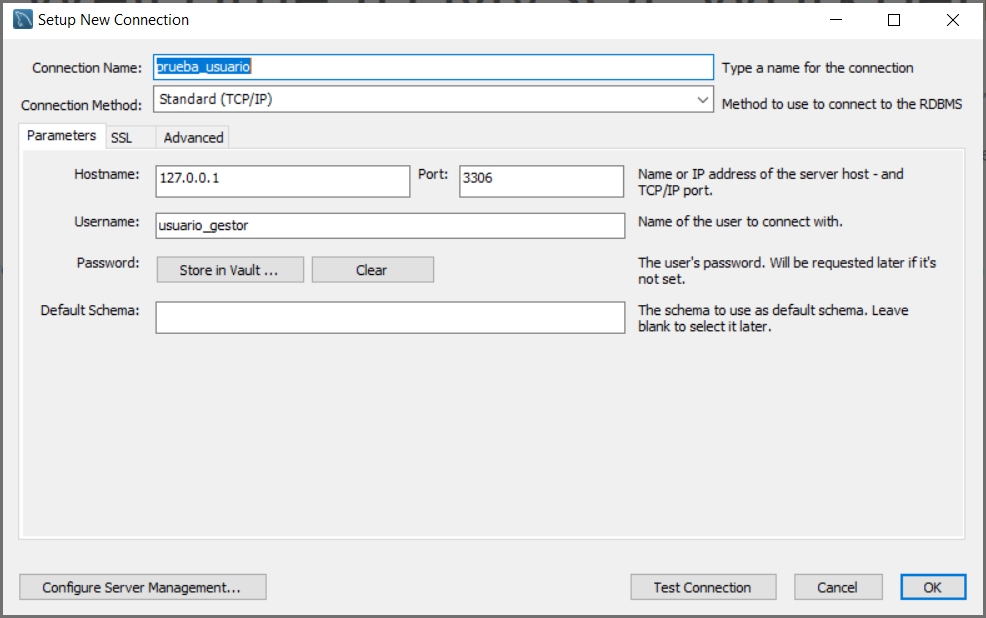
\includegraphics[width=\textwidth]{figs/gestion-usuarios/nueva_conexion_usr.PNG}
    \caption{Creación de la nueva conexión para el usuario \texttt{usuario\_gestor}.}
    \label{fig:nueva-conexion}
\end{figure}

Tras esto, debemos conectarnos al servidor usando la conexión previamente configurada (Figura \ref{fig:eleccion-conexion}).

\begin{figure}[H]
    \centering
    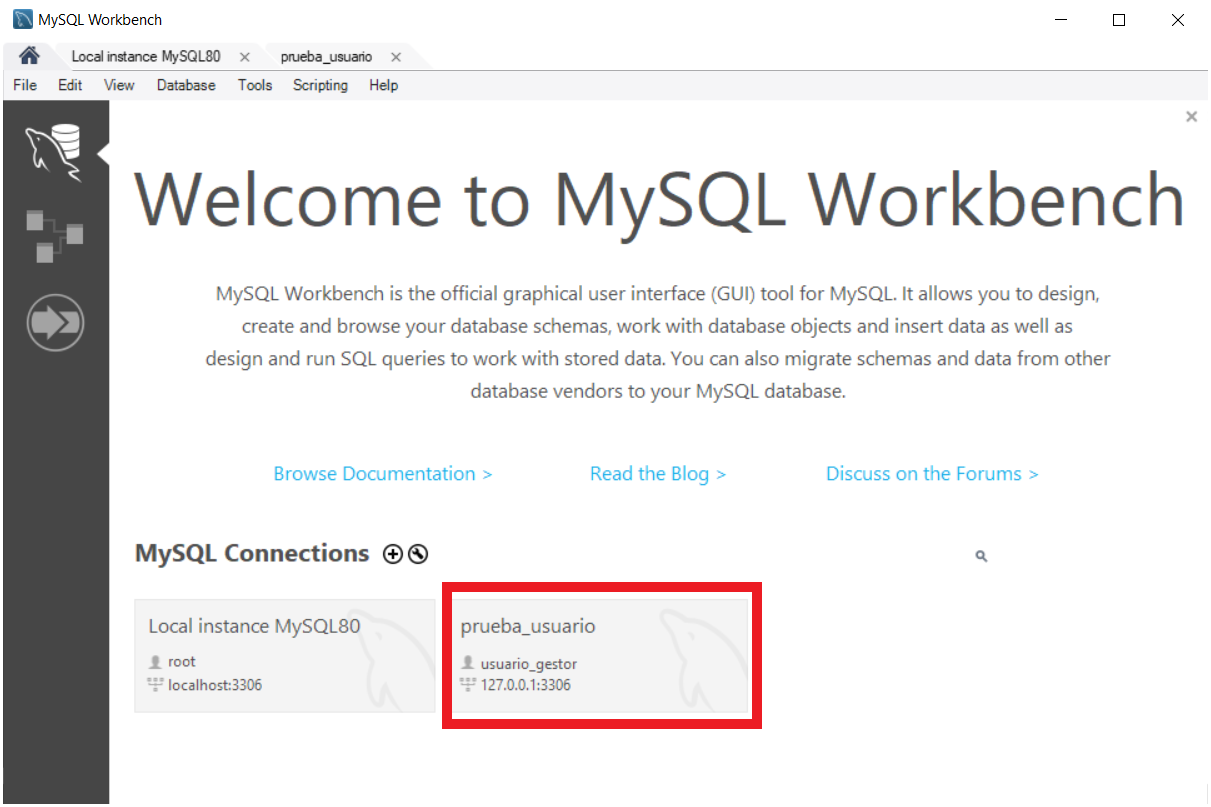
\includegraphics[width=\textwidth]{figs/gestion-usuarios/elegir_conexion_usr.PNG}
    \caption{Elección de la conexión con el nuevo usuario.}
    \label{fig:eleccion-conexion}
\end{figure}

Si prestamos atención al apartado \texttt{schemas}, podremos observar que ahora únicamente está disponible la base de datos \texttt{peliculas}, que es a la que le hemos concedido permisos al usuario \texttt{usuario\_gestor} (Figura \ref{fig:bbdd-disp}).

\begin{figure}[H]
    \centering
    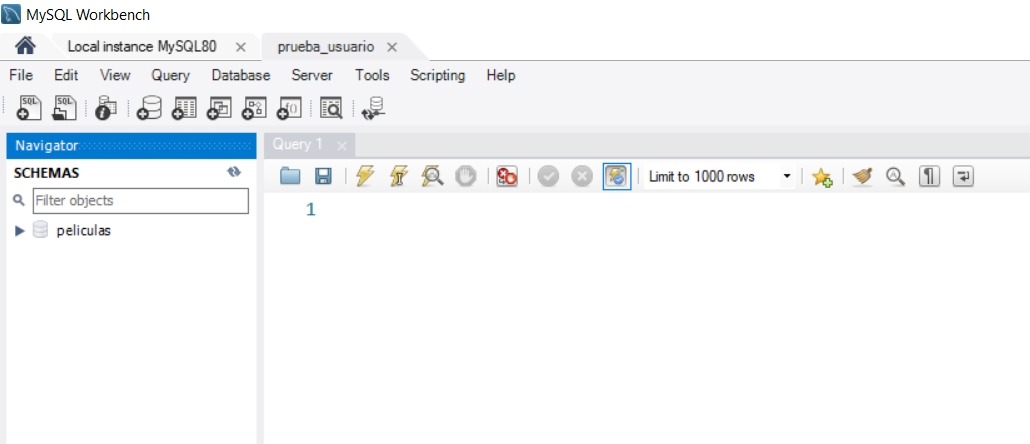
\includegraphics[width=\textwidth]{figs/gestion-usuarios/schemas_disponibles_usr.PNG}
    \caption{Bases de datos disponibles para el usuario \texttt{usuario\_gestor}}.
    \label{fig:bbdd-disp}
\end{figure}

A continuación efectuaremos diferentes operaciones para comprobar que los permisos funcionan correctamente.

En primer lugar, probaremos a ver los registros existentes en la tabla \texttt{actor} (Figura \ref{fig:select}):

\begin{figure}[H]
    \centering
    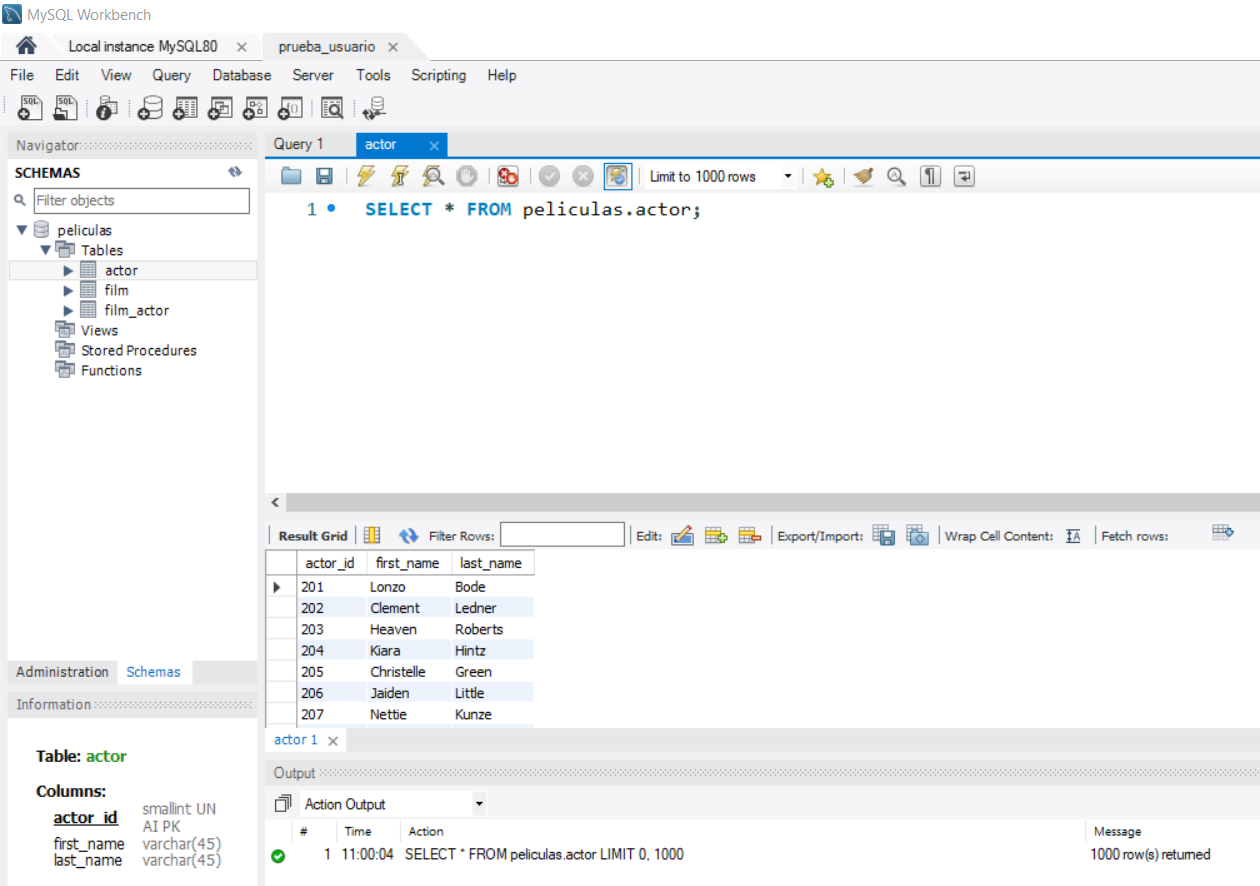
\includegraphics[width=\textwidth]{figs/gestion-usuarios/select_usr.PNG}
    \caption{Selección de los registros de la tabla \texttt{actor}.}
    \label{fig:select}
\end{figure}

Ahora probaremos a modificar el nombre del actor con \texttt{actor\_id = 201} (Figura \ref{fig:update}):

\begin{figure}[H]
    \centering
    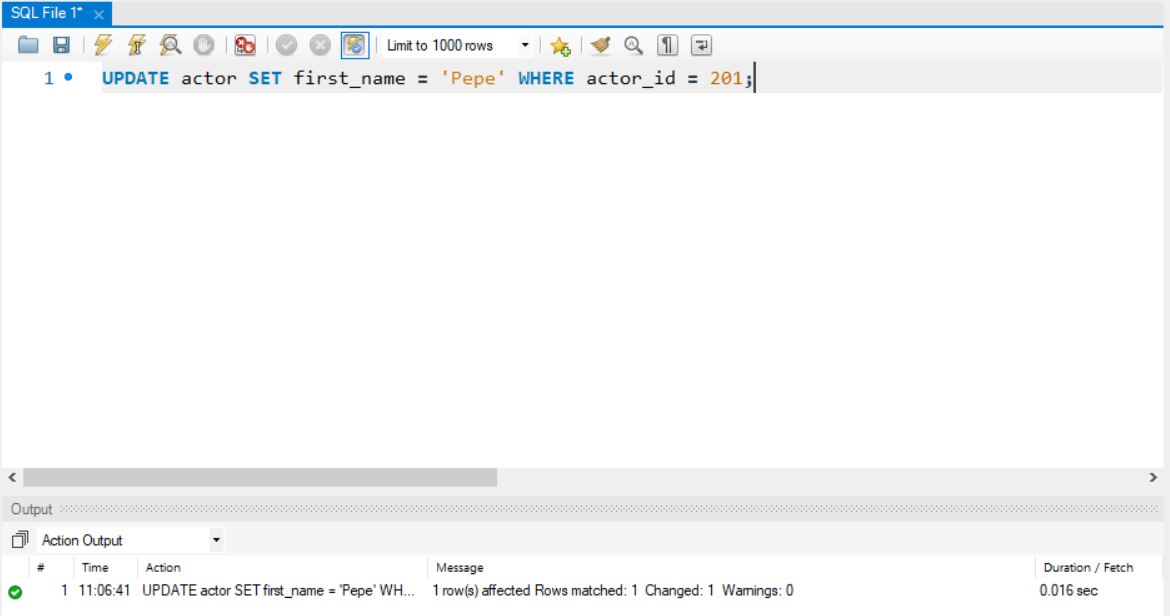
\includegraphics[width=\textwidth]{figs/gestion-usuarios/update_usr.PNG}
    \caption{Elección de la conexión con el nuevo usuario.}
    \label{fig:update}
\end{figure}

Como podéis comprobar, éstas operaciones concluyen con éxito, ya que el usuario \texttt{usuario\_gestor} con el que nos hemos conectado dispone de dichos privilegios (Figura \ref{fig:grants-usuario})

\begin{figure}[H]
    \centering
    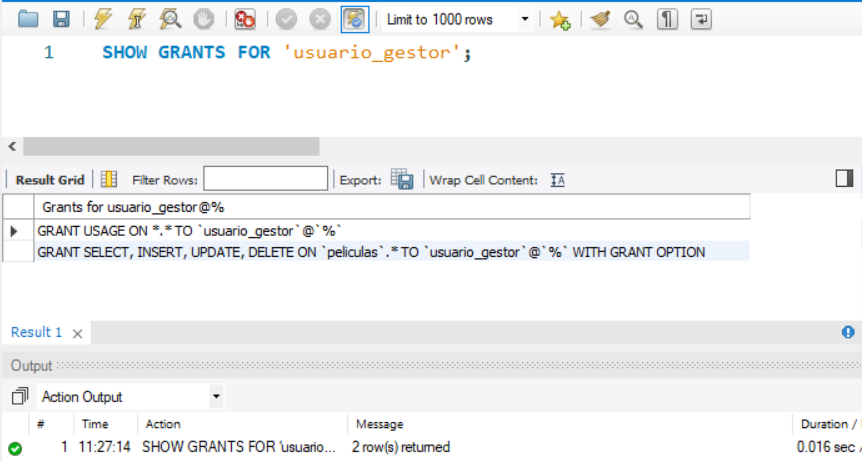
\includegraphics[width=\textwidth]{figs/gestion-usuarios/grants_usuario.PNG}
    \caption{Privilegios del usuario \texttt{usuario\_gestor}.}
    \label{fig:grants-usuario}
\end{figure}

Fijaos que la segunda fila indica los privilegios que le hemos otorgado al usuario, pero en la primera fila aparece:

\texttt{GRANT USAGE ON *.* TO `usuario\_gestor` @ `\%`}


Esto no indica que tenga permisos en todos los schemas y tablas, sino todo lo contrario. De acuerdo al manual de MySQL:

\begin{quote}
    \textit{The USAGE privilege specifier stands for ``no privileges.'' It is used at the global level with GRANT to modify account attributes such as resource limits or SSL characteristics without affecting existing account privileges.}
\end{quote}

Es decir, es la forma de MySQL de indicar que existe un usuario, pero no tiene ningún privilegio. 

Una vez aclarado esto, vamos a comprobar que efectivamente nuestro usuario no tiene determinados permisos.

Vamos a intentar borrar una tabla:

\begin{figure}[H]
    \centering
    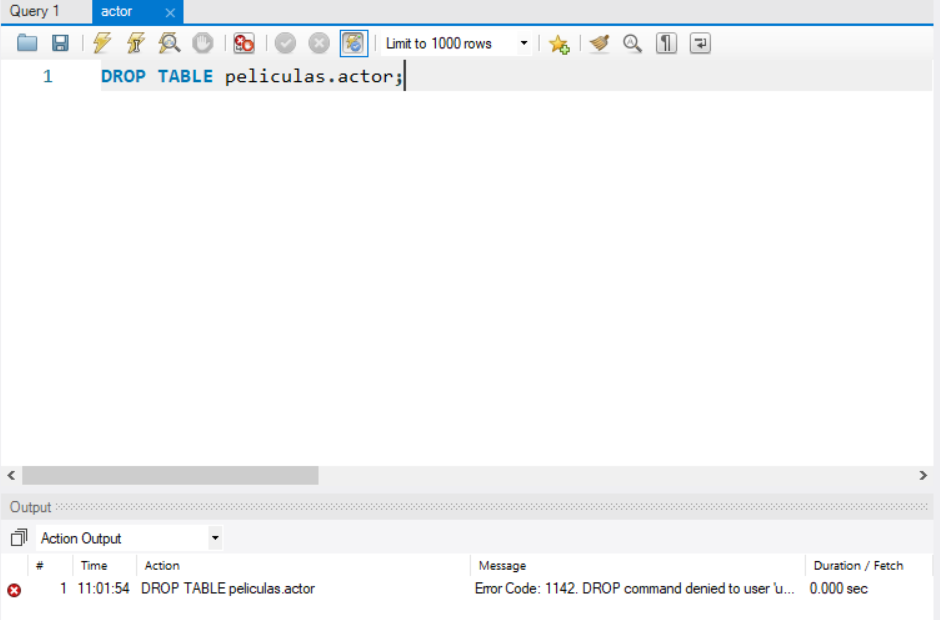
\includegraphics[width=\textwidth]{figs/gestion-usuarios/drop_usr.PNG}
    \caption{Borrado de una tabla.}
    \label{fig:borrar}
\end{figure}

Como podéis observar se produce un error debido a que el privilegio \texttt{DROP} es denegado al usuario \texttt{usuario\_gestor}, tal y como debe ser en base a los privilegios que hemos establecido.

Vamos a probar ahora a crear una tabla:


\begin{figure}[H]
    \centering
    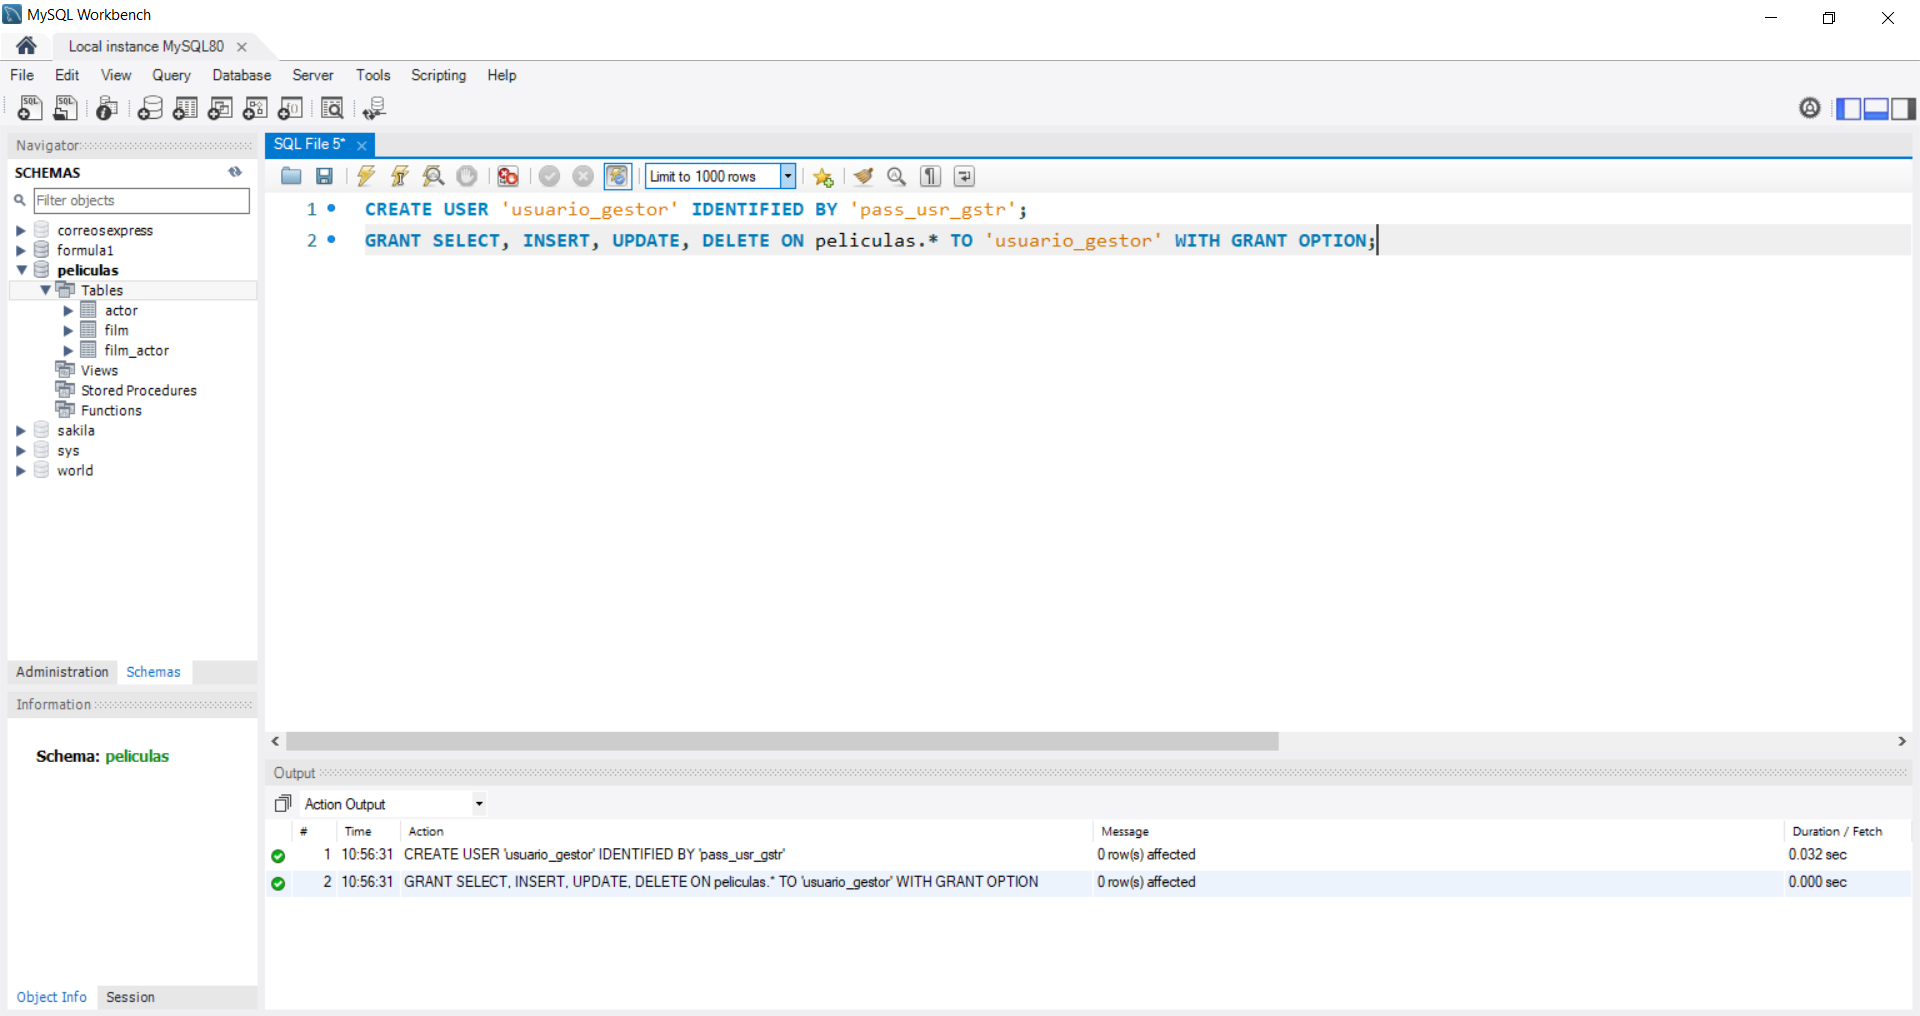
\includegraphics[width=\textwidth]{figs/gestion-usuarios/creacion_usr.PNG}
    \caption{Creación de una tabla.}
    \label{fig:crear}
\end{figure}

De nuevo, nuestro usuario no dispone de los permisos necesarios, por lo que no es posible borrarla.

\subsection*{Gestión de usuarios mediante MySQL Workbench}

También es posible gestionar los usuarios mediante interfaz gráfica. En esta ocasión, le revocaremos el permiso de modificación a nuestro usuario. Para ello, deberemos ir a \textit{Server} $\rightarrow$ \textit{Users and privileges}.

Si entráis desde el usuario \texttt{usuario\_gestor} os encontraréis con que no disponéis de los permisos adecuados (Figura \ref{fig:gestor-usuario}):

\begin{figure}[H]
    \centering
    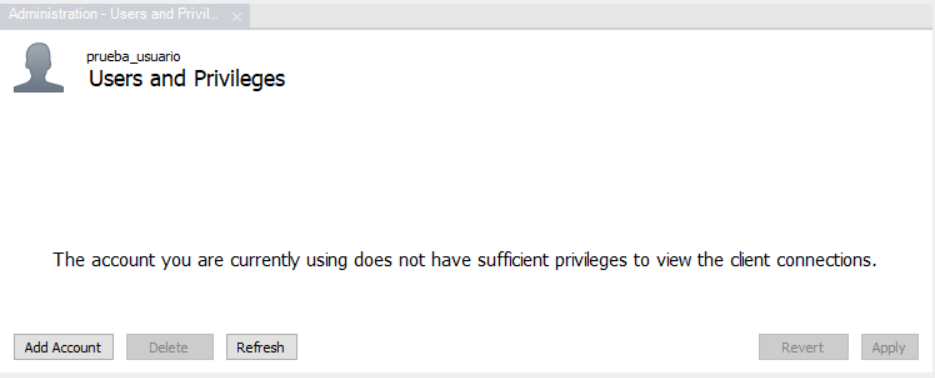
\includegraphics[width=1\linewidth]{figs/gestion-usuarios/gestion-no-permisos.png}
    \caption{El usuario \texttt{usuario\_gestor} no dispone de los permisos adecuados para gestionar usuarios.}
    \label{fig:gestor-usuario}
\end{figure}

Por tanto, deberéis utilizar una conexión como \texttt{root} para llevar a cabo esta tarea. En ese caso, deberíamos ver algo como esto (Figura \ref{fig:gestor-root}):

\begin{figure}[H]
    \centering
    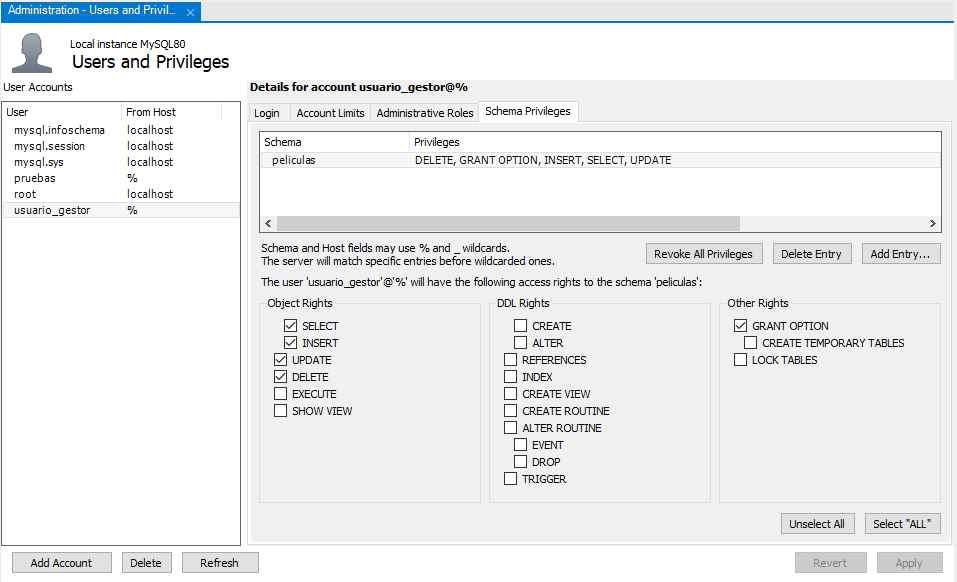
\includegraphics[width=1\linewidth]{figs/gestion-usuarios/gestor-usuarios-root.png}
    \caption{El usuario \texttt{root} sí que dispone de los permisos necesarios.}
    \label{fig:gestor-root}
\end{figure}

Ahora, revocaremos el permiso de \texttt{UPDATE} para el usuario \texttt{usuario\_gestor} des-seleccionando la opción \texttt{UPDATE} y haciendo click en \textit{Apply}.

Si ahora volvemos a conectarnos como \texttt{usuario\_gestor} y probamos a modificar el nombre del actor con \texttt{actor\_id = 201} como hicimos antes, comprobaremos que ya no tenemos permiso (Figura \ref{fig:usr_update_revocado}):

\begin{figure}[H]
    \centering
    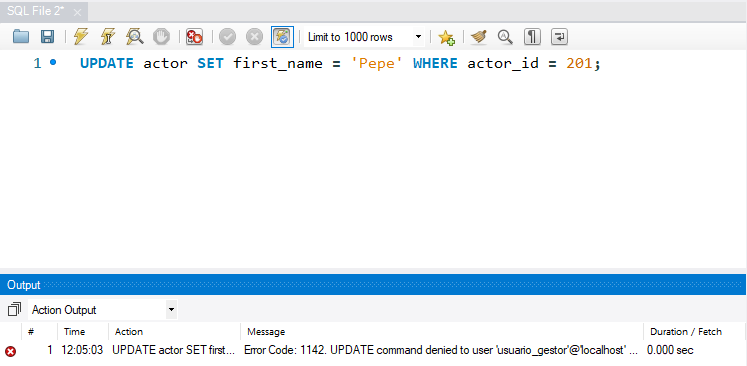
\includegraphics[width=1\linewidth]{figs/gestion-usuarios/usr_update_revocado.png}
    \caption{El usuario \texttt{usuario\_gestor} ya no dispone de permisos para actualizar registros.}
    \label{fig:usr_update_revocado}
\end{figure}

\end{document}
